\documentclass[12pt,a5paper]{article}
\usepackage[a4paper, margin=2cm]{geometry}
\usepackage[utf8]{inputenc}
\usepackage{amsmath}
\usepackage{amsfonts}
\usepackage{graphicx}
\usepackage{amssymb}
\usepackage{imakeidx}
\usepackage{listings}
\usepackage{multirow}
\usepackage{hyperref}
\usepackage{cancel}
\usepackage{subfloat}
\usepackage{caption}
\usepackage{multirow}
\usepackage{multicol}
\usepackage{color}
\usepackage{setspace}
\usepackage{subfig}
\usepackage{parskip}
\usepackage[spanish,es-tabla]{babel}
\usepackage{fancyhdr}
\usepackage{schemata}
\usepackage{appendix}
\usepackage{lastpage}
\usepackage{float}

\graphicspath{ {images/} }

%Detalles de la estructura,
\fancyhf{}
\renewcommand{\headrulewidth}{0,5pt}
\thispagestyle{plain}
\pagestyle{fancy}
\fancyhead[L]{Procesado óptico y digital de señales e imágenes}
\fancyhead[R]{Práctica 1}
\fancyfoot[C]{Página \thepage\ de \pageref{LastPage}}



\begin{document}

%Portada
\begin{titlepage}
\centering
\rule{16 cm}{2 pt}
{\scshape\Huge Procesado óptico y digital de señales e imágenes \par}
\vspace{2cm}
{\scshape\Large \textbf{Práctica 1:} Caracterización de sistemas de formación de imágenes\par}
\rule{16 cm}{2 pt}
\vfill
{\Large \textbf{Alumnos:}\par Alejandro \textcolor{red}{apellidos} \par Adriana \textcolor{red}{apellidos} \par Carlos España Castaño \par}
{\Large Fecha: 16 de noviembre de 2022 \par}
\end{titlepage}



%Índice,
\tableofcontents



\section{Introducción}
En esta práctica vamos a caracterizar un sistema de formación de imágenes mediante la determinación experimental de su función de transferencia de modulación (MTF). Para ello utilizaremos un método directo (el test de barras) y un método indirecto (el test de borde). \par

El sistema cuya MTF mediremos consiste en un objetivo de microscopio con apertura numérica $NA = 0,25$ y un aumento $10X$ (F10), y una cámara CCD con un tamaño de píxel de $s=4,65 \mu m$. Las imágenes captadas por la cámara se visualizarán en la pantalla del PC.




\section{Resultados experimentales}


\subsection{Medida de la MTF mediante el test de barras (método directo)}

Utilizamos el test USAF 1951:

\begin{figure}[h]
    \centering
    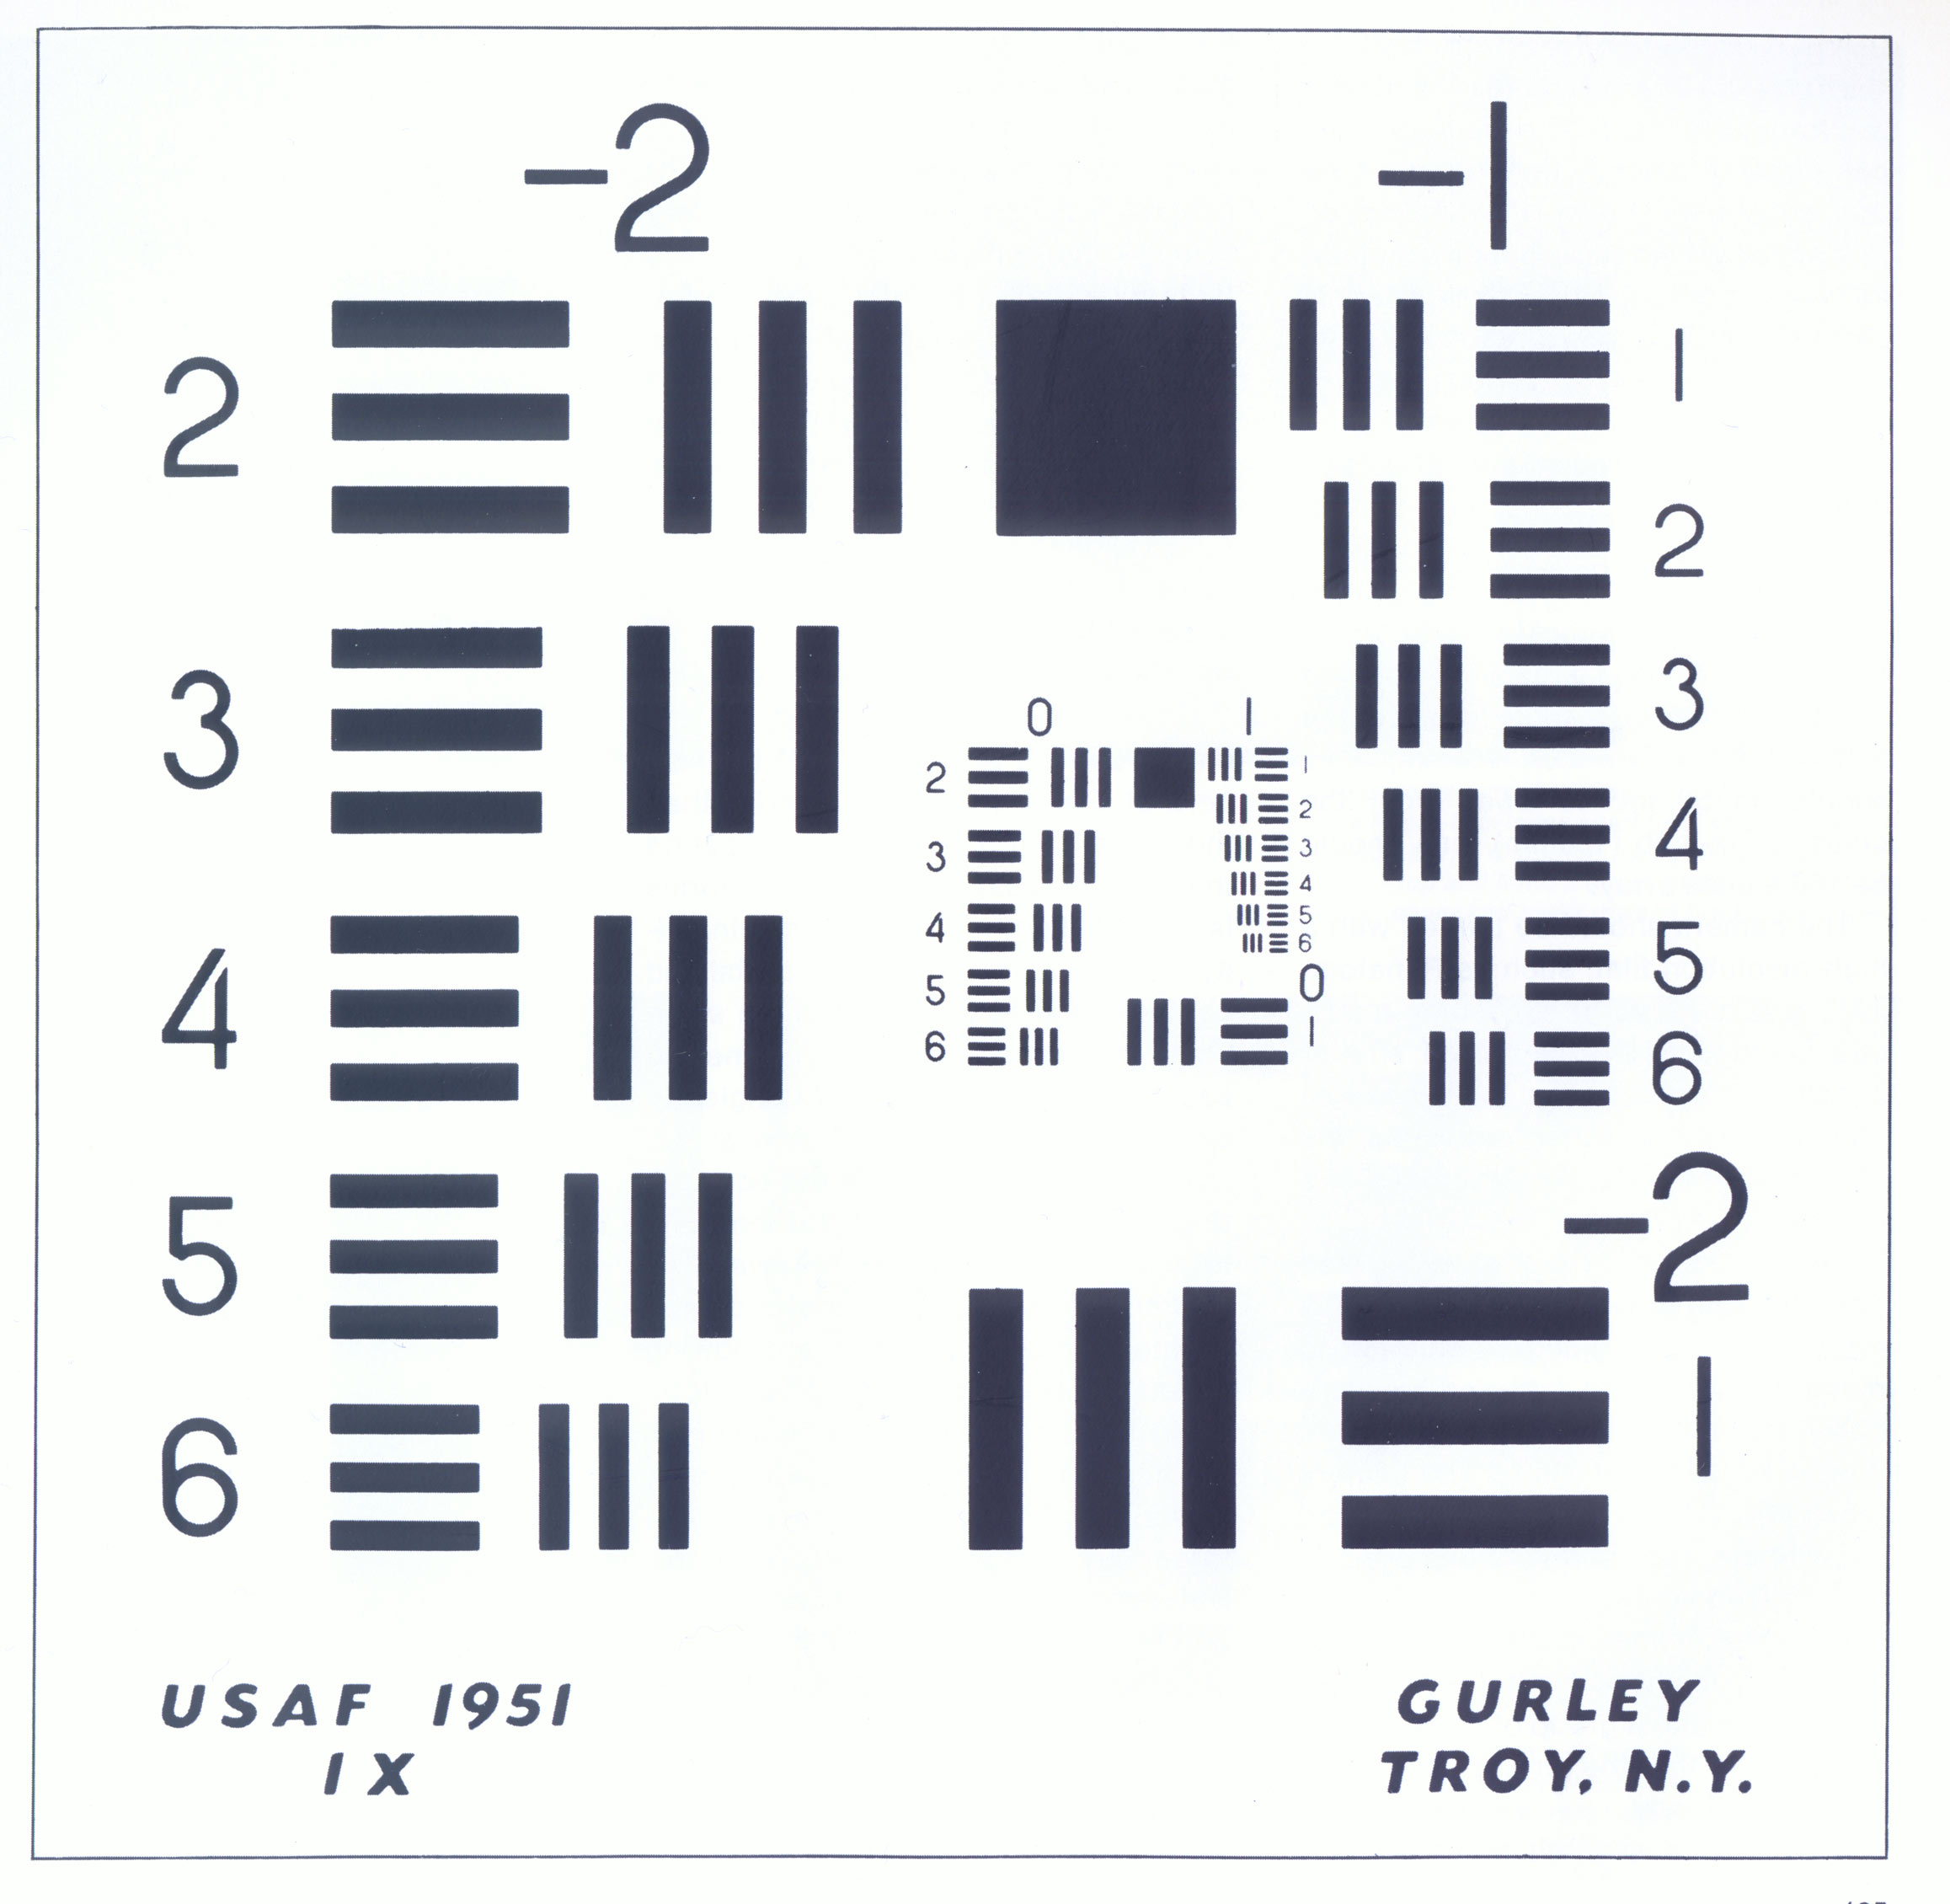
\includegraphics[scale=0.05]{testusaf1951}
    \caption{Test USAF 1951}
    \label{fig:usaf1951}
\end{figure}

En la siguiente tabla se recogen medidas tomadas del perfil de intensidad para distintos conjuntos de barras:

\begin{table}[!ht]
    \centering
    \begin{tabular}{|c|c|c|c|c|c|c|c|c|}
    \hline
        Barras & $y_{min}$ & $y_{max}$ & Contraste & $x_{min}$ & $x_{max}$ & Nºperiodos & Periodo (px) & Frec. ($\frac{ciclos}{mm}$) \\ \hline
        A & 65 & 88 & 0,150 & 4 & 52 & 8 & 6,000 & 304,167 \\ \hline
        B & 65 & 101 & 0,217 & 7 & 73 & 9 & 7,333 & 248,864 \\ \hline
        C & 61 & 108 & 0,278 & 11 & 111 & 11 & 9,091 & 200,750 \\ \hline
        D & 55 & 117 & 0,360 & 4 & 142 & 12 & 11,500 & 158,696 \\ \hline
        E & 58 & 139 & 0,411 & 23 & 183 & 11 & 14,545 & 125,469 \\ \hline
        F & 58 & 142 & 0,420 & 7 & 223 & 12 & 18,000 & 101,389 \\ \hline
        G & 84 & 286 & 0,546 & 19 & 200 & 10 & 18,100 & 100,829 \\ \hline
        H & 65 & 177 & 0,463 & 25 & 251 & 11 & 20,545 & 88,827 \\ \hline
        I & 62 & 191 & 0,510 & 44 & 330 & 10 & 28,600 & 63,811 \\ \hline
        J & 40 & 156 & 0,592 & 15 & 381 & 10 & 36,600 & 49,863 \\ \hline
        K & 35 & 191 & 0,690 & 53 & 463 & 9 & 45,556 & 40,061 \\ \hline
        L & 23 & 156 & 0,743 & 30 & 674 & 11 & 58,545 & 31,172 \\ \hline
        M & 25 & 191 & 0,769 & 32 & 683 & 9 & 72,333 & 25,230 \\ \hline
        N & 18 & 199 & 0,834 & 44 & 596 & 6 & 92,000 & 19,837 \\ \hline
        O & 12 & 182 & 0,876 & 66 & 635 & 5 & 113,800 & 16,037 \\ \hline
        P & 12 & 198 & 0,886 & 66 & 664 & 4 & 149,500 & 12,207 \\ \hline
        Q & 11 & 188 & 0,889 & 98 & 640 & 3 & 180,667 & 10,101 \\ \hline
    \end{tabular}
    \caption{\small Datos del perfil de intensidad. y: intensidad. x: distancia en píxeles}
    \label{table:perfilintensidad}
\end{table}

El contraste se ha obtenido a partir de la expresión:

\begin{equation}
        C = \frac{y_{max} - y_{min}}{y_{max} + y_{min}}
    \label{contraste}
\end{equation}

La frecuencia, en ciclos/mm, se ha calculado como:

\begin{equation}
        u = \frac{1825}{periodo} (ciclos/mm)
    \label{frecuencia}
\end{equation}

Donde el periodo se obtiene dividiendo la diferencia $x_{max} - x_{min}$ entre el número de periodos en ese intervalo.



\subsection{Medida de la MTF mediante el test de borde (método indirecto)}







\newpage

\section{Cuestiones}

\subsection{Cuestión 1}
Sea $H_{c}(u)$ la función de transferencia de un sistema para luz coherente. Escribir la relación entre $H_{c}(u)$ y la función de transferencia del mismo sistema para luz incoherente, $H_{i}(u)$.


\subsection{Cuestión 2}
Para un sistema parecido al usado en la práctica:
\begin{enumerate}
    \item Estimar la frecuencia de corte de la cámara CCD, $u_{c}^{(CCD)}$, en líneas por milímetro.
    
    \item Estimar la frecuencia de corte $u_{c}^{(Obj)}$ del objetivo $10x$ para luz incoherente (la longitud de onda media $\lambda=500nm$.
    
    \item Tomando estos valores y suponiendo que la PSF del objetivo y de la cámara se aproximan por la función $|sinc(ax)|^2$, dibujar la MTF de cada uno de los elementos y del sistema compuesto.
\end{enumerate}


\subsection{Cuestión 3}
Aplicar usando el plugin Deconvolutionlab2 y Image J dos métodos de convolución: Regularized Inverse Filter y Richardson-Lucy a una imagen test obtenida por un sistema con una PSF conocida y diferentes tipos de ruido: Guass y Poisson.


\end{document}